\chapter{Results and Analysis}
\label{Chapter:Results}

\section{Serpent Model}

\subsection{Excess Reactivity and Shutdown Margin}

\begin{figure}[!ht]
    \centering
    \subfloat[\centering Single Misfire]{\includegraphics[width=0.49\textwidth]{Plotter/0.0shutdown7drum/MSNB_geom4}}
    \subfloat[\centering Single Success]{\includegraphics[width=0.49\textwidth]{Plotter/0.0shutdown1drum/MSNB_geom4}}
    \caption[X-Y View of \acs{msnb} - Shut-Down Margin]{X-Y Views of \acs{msnb} with control drums in two shut-down margin failure modes:
    \begin{enumerate*}[label=\alph*)]
        \item Seven drums in least reactive orientation, one drum failed in most reactive orientation; and 
        \item One drum in least reactive orientation, seven drums failed in most reactive orientation; 
    \end{enumerate*}
    }
    \label{fig:Plotter-SDM}
\end{figure}




including burned B4C

\subsection{Neutron Spectra}
\begin{figure}[ht!]
    \centering
    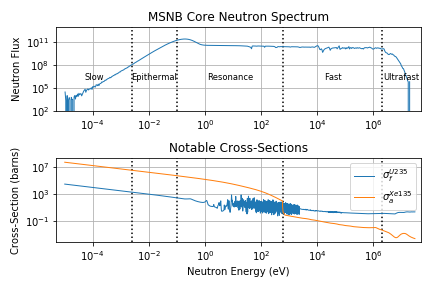
\includegraphics[width=0.9\textwidth]{./Plotter/Detector/Spectrum}
    \caption[\acs{msnb} Neutron Energy Spectrum]{\raggedright \acs{msnb} neutron energy spectrum in core, reflector, and downcomer.}
    \label{fig:Spectrum}
\end{figure}


\subsection{Actuator Curve}\label{sec:actuator}

\section{Multi-physics Simulation}

\subsection{Steady-State}

\subsection{Up-Step}
autonomous
controller tuning
controlled response


\subsection{Down-Step}

\subsection{Start-Up}

\subsection{Shut-Down}

\subsection{Demand-Response}